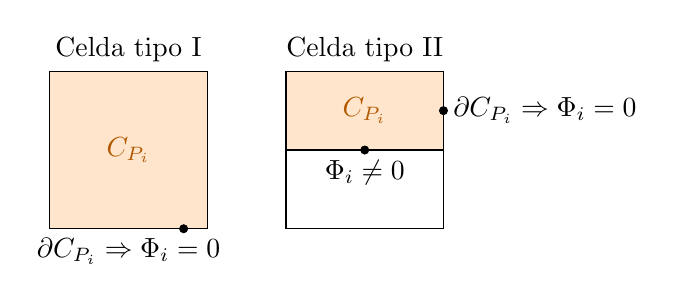
\begin{tikzpicture}
\draw[fill=orange!20!white] (0,0) rectangle (2,2);
\node[orange!70!black] at (1,1) {$C_{P_i}$};
\node[below] at (1,0) {$\partial C_{P_i} \Rightarrow \Phi_i = 0$};
\node[draw,circle,inner sep=1pt,black,fill=black] at (1.7,0) {};
\node[above] at (1,2) {Celda tipo I};

\draw[fill=white] (3,0) rectangle (5,2);
\draw[fill=orange!20!white] (3,1) rectangle (5,2);
\node[draw,circle,inner sep=1pt,black,fill=black] at (4,1) {};
\node[orange!70!black] at (4,1.5) {$C_{P_i}$};
\node[right] at (5,1.5) {$\partial C_{P_i} \Rightarrow \Phi_i = 0$};
\node[draw,circle,inner sep=1pt,black,fill=black] at (5,1.5) {};
\node[below] at (4,1) {$\Phi_i \neq 0$};
\node[above] at (4,2) {Celda tipo II};

\end{tikzpicture}